
\chapter{Estado del arte y fundamentos teóricos}\label{estadoArte}

En este capítulo analizaré el estado actual del tema a tratar, junto con una pequeña revisión bibliográfica y algunos conceptos teóricos necesarios. También profundizaré un poco más en las representaciones lineales comentadas en el Capítulo \ref{introduccion}, así como los distintos paquetes software existentes y sus limitaciones. 

\section{Revisión bibliográfica} \label{revision_bib}
Para el estudio de los trabajos relacionados y búsqueda de bibliografía se han consultado fuentes como IEEE Xplore, ACS Publications, o Journal of Chemical Information and Computer Sciences, entre otras. En la Figura \ref{fig:revisionBibliografica} se exponen los resultados de un breve estudio bibliográfico sobre la literatura existente de los temas del proyecto. 

Todo comienza en 1988 con la publicación de David Weininger \cite{weininger_smiles_1988}, presentando SMILES como un nuevo formato de representación lineal, a partir de ahí y hasta día de hoy, fueron aumentando las publicaciones alrededor de SMILES. Sin embargo, vemos que apenas existe literatura para temas más específicos dentro de este área, como la canonización de las cadenas SMILES o la organometálica (ver Secciones \ref{teoria:representaciones_lineales} y \ref{teoria:ogm}). Además, si nos paramos a revisar las publicaciones existentes vemos que apenas ninguna coincide con los objetivos de este proyecto, y mucho menos hacen alguna propuesta de cómo darles solución. Los datos de las publicaciones se han recopilado a través de \textit{Scopus}\footnote{\url{https://www.elsevier.com/es-es/solutions/scopus}}\footnotecomma\footnote{\url{https://biblioteca.ugr.es/investigacion/herramientas-apoyo/evaluacion-publicaciones/scopus}} con las siguientes consultas, donde CHEM y COMP hacen referencia a chemistry y computer science respectivamente: 
\begin{itemize}
    \item {\footnotesize \textit{(SUBJAREA(CHEM) AND TITLE-ABS-KEY(smiles))}} 
    \item {\footnotesize \textit{((SUBJAREA(CHEM) OR SUBJAREA(COMP)) AND TITLE-ABS-KEY(smiles AND canonical))}}
    \item {\footnotesize \textit{(SUBJAREA(CHEM) AND TITLE-ABS-KEY(smiles AND organometallic))}}
\end{itemize}

\begin{figure}[h!]
        \centering
        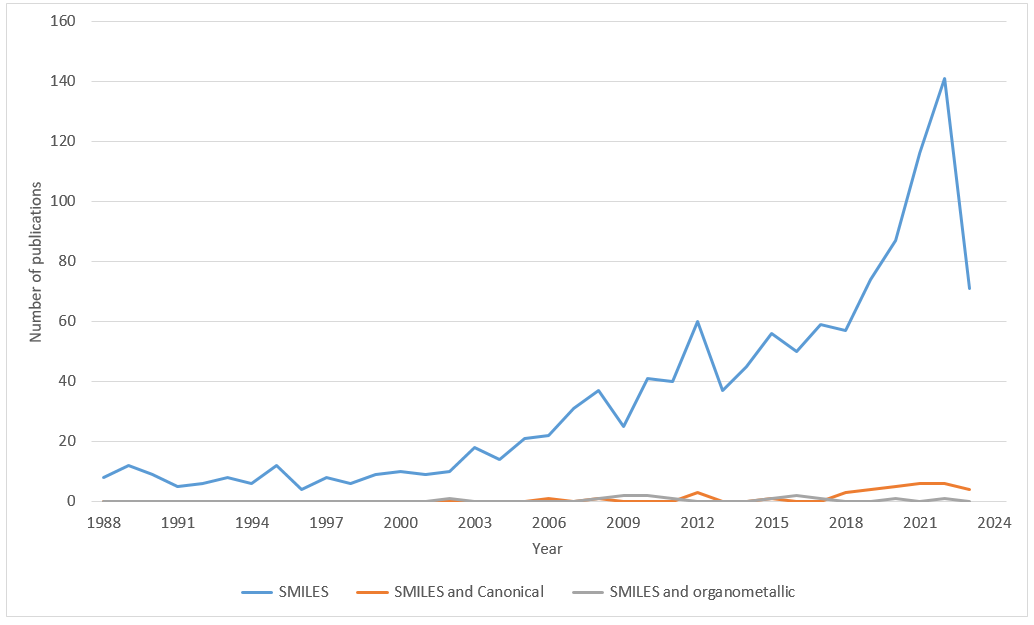
\includegraphics[scale=0.5]{imagenes/estado_arte/revisionBibliografica.png}
        \caption{Comparativa del número de artículos publicados por año según las palabras clave de la búsqueda. Imagen de elaboración propia. Datos extraídos de \emph{Scopus}.}
        \label{fig:revisionBibliografica}
    \end{figure}


\section{Fundamentos teóricos}

\subsection{Moléculas y sus representaciones}

Existen numerosas formas de representar una molécula. La más usada es la representación del grafo molecular, siendo capaces de ver rápidamente las conexiones entre átomos. El grafo molecular es un tipo de grafo no dirigido en el que los nodos están etiquetados y las aristas ponderadas. Los nodos se etiquetan según el tipo de átomo que representen, utilizando su símbolo químico: si es un carbono (C), oxígeno (O), nitrógeno (N), cloro (Cl), etc; mientras que a las aristas se le atribuyen pesos según su tipo de enlace: simple, doble, triple o aromático. El concepto de aromaticidad es particularmente importante en química. El compuesto aromático por excelencia es el benceno, conformado por una serie de electrones deslocalizados de tal manera que no se pueden describir sus enlaces con enlaces simples o dobles, sino con una alternancia de ambos o directamente usando la forma resonante (visualizada con una curva, Figura \ref{fig:aromatico_benceno}).

\begin{figure}[h!]
    \centering
    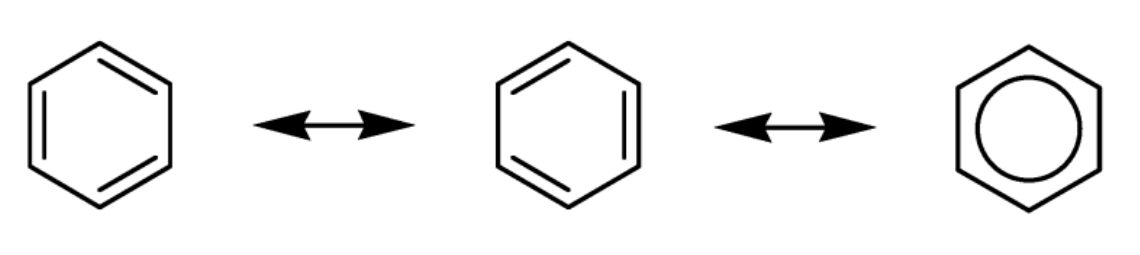
\includegraphics[scale=0.35]{imagenes/estado_arte/teoria/benceno.png}
    \caption{Alternativas en la representación del benceno de acuerdo a su aromaticidad. Anillo de 6 carbonos con electrones deslocalizados. Imagen extraída parcialmente de \cite{iupac_manual}.}
    \label{fig:aromatico_benceno}
\end{figure}

Hay varias opciones de visualización. Los carbonos por ejemplo, por lo general únicamente se representan si son terminales (último átomo de la cadena), aunque podrían representarse también los carbonos en mitad de una cadena o no hacerlo aun siendo terminales. Los hidrógenos tampoco se representan ya que la mayoría de ellos son implícitos, es decir, se usan para llenar las valencias sin usar de cada uno de los átomos de la molécula. Según la Teoría de Enlaces de Valencia, a cada átomo se le asigna una valencia típica (la más frecuente, sin tener en cuenta los estados de oxidación), así por ejemplo: el carbono tiene una valencia de 4, el oxígeno de 2, el nitrógeno de 3, etc \cite{vbt, brown_chemoinformaticsintroduction_2009}. Se muestra en la Figura \ref{fig:grafo_molecular_caf_asp} dos ejemplos de moléculas representadas por su grafo molecular.

\begin{figure}[h!]
\centering
\begin{subfigure}{.5\textwidth}
  \centering
  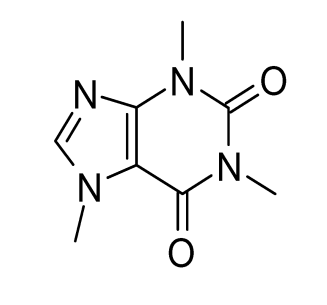
\includegraphics[width=.7\linewidth]{imagenes/estado_arte/teoria/cafeina.png}
  \caption{Cafeína}
\end{subfigure}%
\begin{subfigure}{.5\textwidth}
  \centering
  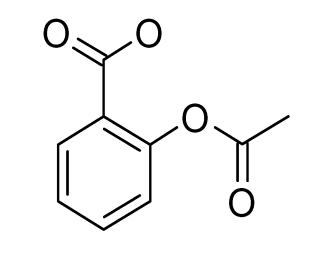
\includegraphics[width=.7\linewidth]{imagenes/estado_arte/teoria/aspirina.png}
  \caption{Aspirina}
\end{subfigure}
\caption{Grafo molecular sin hidrógenos de \textbf{(a)} la cafeína y \textbf{(b)} la aspirina. Imágenes extraídas de \cite{brown_chemoinformaticsintroduction_2009}.}
\label{fig:grafo_molecular_caf_asp}
\end{figure}


Como representación alternativa al grafo molecular tenemos la tabla de conexiones —que es en realidad una representación matricial del grafo molecular—, muy utilizada por los formatos de archivo más comunes para almacenar moléculas, SDF (Structural Data File), MOL2 o CML (Chemical Markup Languaje) entre otros. La tabla de conexiones separa la información de los átomos y los enlaces en dos bloques dentro del fichero. Por último, tenemos del formato de fichero '\textit{.smi}', en donde se pueden almacenar 1 o múltiples cadenas SMILES. representado cada línea del fichero una cadena SMILES distinta.

\begin{figure}[h!]
    \centering
    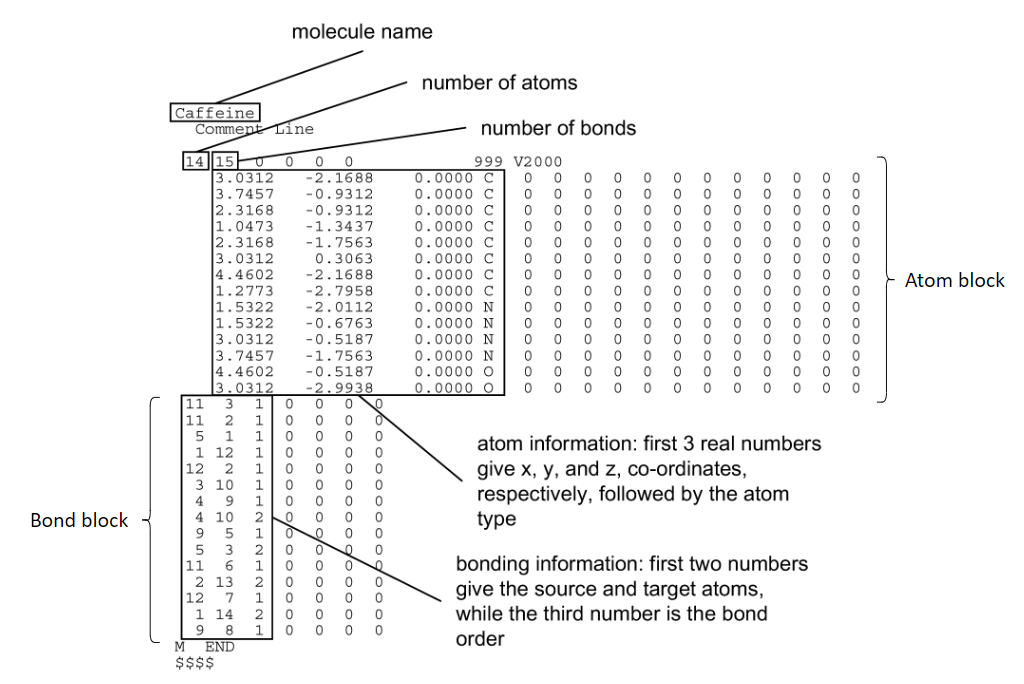
\includegraphics[scale=0.5]{imagenes/estado_arte/teoria/conection_table.png}
    \caption{Tabla de conexiones para la cafeína en un fichero SDF. Imagen extraída de \cite{brown_chemoinformaticsintroduction_2009}.}
    \label{fig:conection_table}
\end{figure}

\subsection{Representaciones lineales} \label{teoria:representaciones_lineales}
En la Sección \ref{motivacion} ya se expone la necesidad de las representaciones lineales, y se nombran 3 principalmente: SMILES, InChI, y SELFIES. Para entenderlas mejor, se pasa a describir la sintaxis de cada una de ellas.

\subsubsection{SMILES, Simplified Molecular-Input Line-Entry System}

SMILES representa una molécula mediante una cadena de caracteres con sus átomos. Las reglas para describir una cadena SMILES son las siguientes:
\begin{itemize}
    \item Los \textit{átomos} se representan por su símbolo atómico, normalmente en mayúsculas.
    \item Los \textit{enlaces} se especifican mediante los caracteres ``$-$'', ``$=$'' y ``\#'' para enlaces simples, dobles y triples respectivamente, aunque los simples no se suelen representar al ser implícitos.
    \item Las \textit{ramificaciones} se especifican entre paréntesis, pudiendo ser anidados.
    \item Los \textit{ciclos} se representan mediante un número común que aparece tras los átomos de apertura y cierre del ciclo, indicando los átomos que se conectan entre sí (como si se rompiera el ciclo y los números lo volvieran a unir).
    \item Las \textit{estructuras aromáticas} se especifican escribiendo los átomos que la componen en minúscula. Por ejemplo, el benceno `c1ccccc1'. Se suele preferir esta forma aromática sobre la convencional con dobles y simples enlaces `C1=CC=CC=C1'.
\end{itemize}

Aquí se han recogido los aspectos básicos sobre la sintaxis de SMILES. Para más información acerca de la especificación de SMILES, ver \cite{smiles_tuto, weininger_smiles_1988}. Igualmente, se hablará más sobre SMILES y se verán numerosos ejemplos durante el resto del documento.

\subsubsection{InChI, International Chemical Identifier}

Un identificador InChI es una cadena de símbolos legible por máquina que permite a un ordenador representar el compuesto de forma totalmente inequívoca. Además, la estructura original puede recuperarse a partir de su InChI a través del software adecuado. Como vemos en la Figura \ref{fig:inchi_ejemplo}, no es directamente inteligible para el lector humano. InChI representa las diversas características de una estructura química de forma jerárquica, por capas \cite{heller_inchi_2015, heller_inchi_resumed_2013}. Cada una de las capas están separadas por `/', y dependiendo de la molécula aparecerán unas capas u otras; cada capa puede tener varias subcapas dedicadas a una propiedad determinada de la molécula (consultar \cite{heller_inchi_2015, heller_inchi_resumed_2013}). Las capas son las siguientes: 
\begin{itemize}
    \item Capa principal
    \begin{itemize}
        \item Fórmula molecular
        \item Conectividades entre átomos
    \end{itemize}
    \item Especificación de cargas
    \item Información sobre estereoquímica
    \item Información sobre isótopos
\end{itemize}

\begin{figure}[h!]
    \centering
    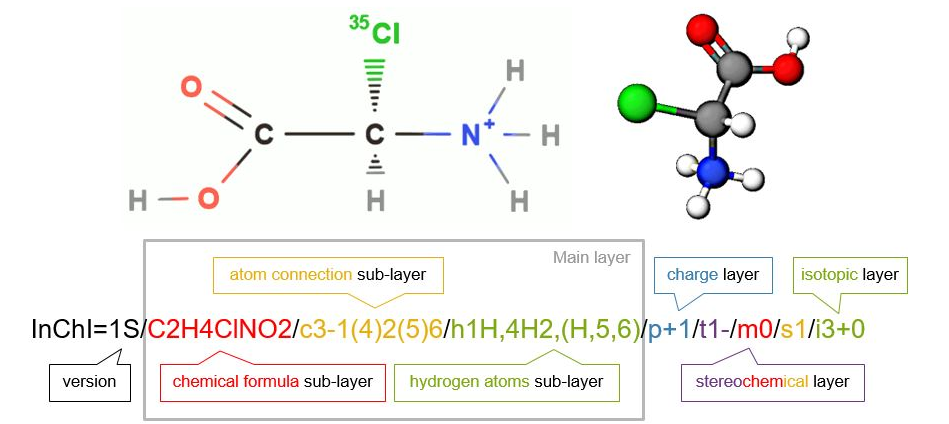
\includegraphics[scale=0.48]{imagenes/estado_arte/teoria/inchi_ejemplo.png}
    \caption{Representación del grafo molecular y modelo 3D, junto con su InChI para el \textit{[(R)-carboxy(chloro)methyl]azanium}, obtenida a partir del \textit{2-$(\prescript{35}{}{Cl})$chloro-R-glycine}. Imagen extraída de \cite{libretext_linenotation}.}
    \label{fig:inchi_ejemplo}
\end{figure}


Aunque InChI es una cadena única que identifica una estructura química, su longitud aumenta con el tamaño de la estructura a representar. Una estructura con más de 100 átomos da como resultado un InChI muy largo. Se vio la necesidad por tanto de desarrollar una versión compacta de InChI para que los motores de búsqueda de las bases de datos fueran efectivos. Esto es InChIKey, una cadena con una longitud fija de 27 caracteres, calculada en base a algoritmos de hashing. El problema de InChIKey es que se pierde la capacidad de recuperar la estructura a la que pertenece, así que para saber la molécula de un determinado InChIKey es necesario hacer una búsqueda en las bases de datos.

\subsubsection{SELFIES, SELF-referencIng Embedded Strings}

SELFIES es una representación basada en una secuencia de tokens con restriciones semánticas. SELFIES en sí mismo es una gramática formal de Chomsky de tipo 2, reforzada con funciones recursivas autorreferenciadas asegurar la generación de grafos sintáctica y semánticamente válidos \cite{krenn_selfies_example}. La gramática de SELFIES está diseñada específicamente con el objetivo de eliminar moléculas sintáctica y semánticamente inválidas para su uso en tareas generativas.
La secuencia va formándose en varios pasos o estados, utilizando unas reglas de derivación (consultar las reglas en \cite{selfies_derivation_rules, krenn_selfies_example}).
Lo más importante a saber para entender una secuencia SELFIES son las siguientes pautas:
\begin{itemize}
    \item Cualquier token de la cadena debe ir entre corchetes.
    \item Los átomos se especifican con su símbolo atómico, precedido si es necesario del tipo de enlace (`$=$', `\#').
    \item Para la especificación de ramas y ciclos, en lugar de tener un número de apertura y cierre como SMILES, solamente se usa un token en una posición, y el token siguiente define la longitud de la rama o ciclo. Tanto ramas como ciclos siempre empiezan con `[Branch1]' o `[$<B>$Ring1]' respectivamente, y los tokens que indican la longitud se muestran en la Tabla \ref{tab:tokens_longitud}.
    \begin{itemize}
        \item En el caso de las ramas, el token de longitud indica que los ($Q+1$) tokens siguientes son los que forman parte de la rama (incluyendo otros tokens de rama o ciclo).
        \item En el caso de los ciclos, el token de longitud indica que el átomo actual se conecta con un enlace de tipo $<B>$ (` ', `$=$' o `\#') al átomo ($Q+1$) posiciones previas (excluyendo tokens de ramas o ciclos). 
    \end{itemize}
\end{itemize}

\begin{table}[h!]
    \centering
    \small
    \begin{tabular}{|ll|ll|}
       \toprule 
       Q & Token        & Q     & Token \\
       \midrule
       0 & [C]          & 8     & [\#Branch2] \\
       1 & [Ring1]      & 9     & [O] \\
       2 & [Ring2]      & 10    & [N] \\
       3 & [Branch1]    & 11    & [=N] \\
       4 & [=Branch1]   & 12    & [=C] \\
       5 & [\#Branch1]  & 13    & [\#C] \\
       6 & [Branch2]    & 14    & [S] \\
       7 & [=Branch2]   & 15    & [P] \\
       \midrule
       \multicolumn{4}{|c|}{Cualquier otro token implica índice 0}\\
       \bottomrule
    \end{tabular}
    \caption{Lista de símbolos SELFIES con las longitudes que representan cuando aparecen tras una rama o ciclo. Está basado en un sistema hexadecimal y números mayores se pueden mapear si se utilizan los siguientes $n$ símbolos. Tabla elaborada en base a \cite{SELFIES}.}
    \label{tab:tokens_longitud}
\end{table}

% En la Figura \ref{fig:selfies_ejemplo} vemos un ejemplo de la derivación de SELFIES.
\begin{figure}[h!]
    \centering
    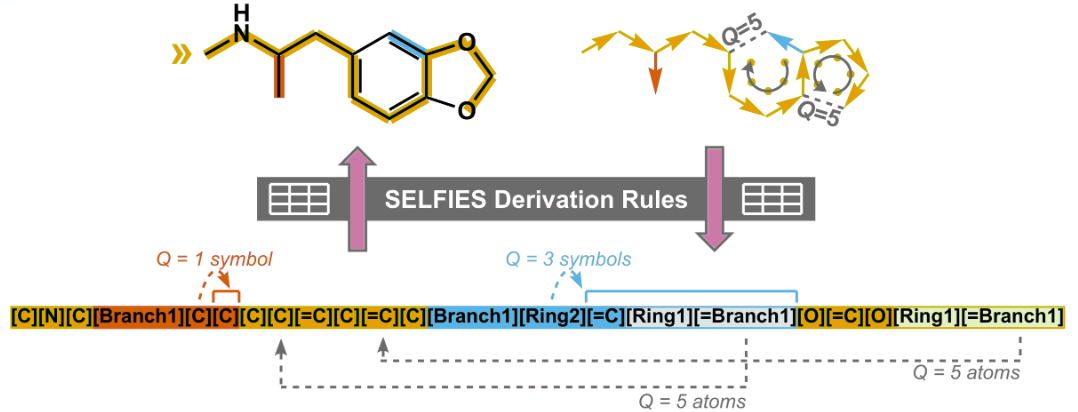
\includegraphics[scale=0.43]{imagenes/estado_arte/teoria/selfies_ejemplo.png}
    \caption{SELFIES para la estructura molecular de \textit{3,4-methylenedioxy methamphetamine} (MDMA). Imagen extraída de \cite{SELFIES}.}
    \label{fig:selfies_ejemplo}
\end{figure}



\subsection{Organometálica} \label{teoria:ogm}

La organometálica es una rama de la química que se dedica al estudio de compuestos organometálicos, es decir, aquellos que contienen enlaces metal-carbono. Este tipo de compuestos normalmente se clasifican dentro de la química de coordinación, pero con algunas diferencias. Los compuestos de coordinación tienen un metal coordinado (ligado) a cualquier cosa, por lo general `restos' de alguna reacción previa y que no necesariamente deben ser orgánicos. Por tanto, no todos los compuestos de coordinación son compuestos organometálicos, pero sí podemos considerar todos los organometálicos como de coordinación. En una reacción por ejemplo, lo importante es que exista una unión metal-carbono en algún punto para considerarla dentro de la organometálica.
Cuando hablamos de `metales', se están considerando los metales de transición, ya que al tener orbitales `\textit{d}' disponibles son muy propensos a este tipo de enlaces con ligandos. Estos abarcan desde el grupo 3 hasta el 12 en la tabla periódica, del escandio (Sc) al zinc (Zn) a lo largo de los periodos 4 al 7\footnote{explicaciones dadas por los expertos}.


Dentro de los compuestos organometálicos, los metalocenos son muy comunes y reconocibles. Estos se caracterizan por un catión metálico central, usualmente de un metal de transición, y dos ligandos orgánicos llamados ciclopentadienilos (Cp\footnote{en adelante se hará referencia como Cp}). Los ligandos Cp están formados por un anillo de cinco átomos de carbono unidos mediante enlaces covalentes. Estos ligandos Cp se unen al metal central de manera que cada átomo de carbono en el anillo Cp contribuye con un par de electrones pi para formar enlaces con el metal. Debido a la presencia de los enlaces pi, los metalocenos exhiben una gran estabilidad y reactividad química característica, lo que ha llevado a su amplio uso en catálisis y síntesis orgánica. Esta clase de enlaces se denomina \textit{hapticidad}, en donde un grupo de átomos contiguos de un ligando se coordinan a un átomo de metal central. Se utiliza el símbolo griego `eta', $\eta$ con el número de átomos contiguos que se coordinan como superíndice. Para el ferroceno mostrado en la Figura \ref{fig:metalocenos_ejemplos}, serían 2 ligandos de $\eta^{5}$-$C_{5}H_{5}$ (para el lector interesado, revisar la literatura sobre química organometálica \cite{jose_curso_1995, fajarnes_quimica_1997, osorio-yanez_compuestos_2021, organometallic_hypertextbook, libretext_organometallic_2013}). En la siguiente Figura \ref{fig:metalocenos_ejemplos} podemos ver algunos ejemplos:
\begin{figure}[h!]
\centering
\begin{subfigure}{.5\textwidth}
  \centering
  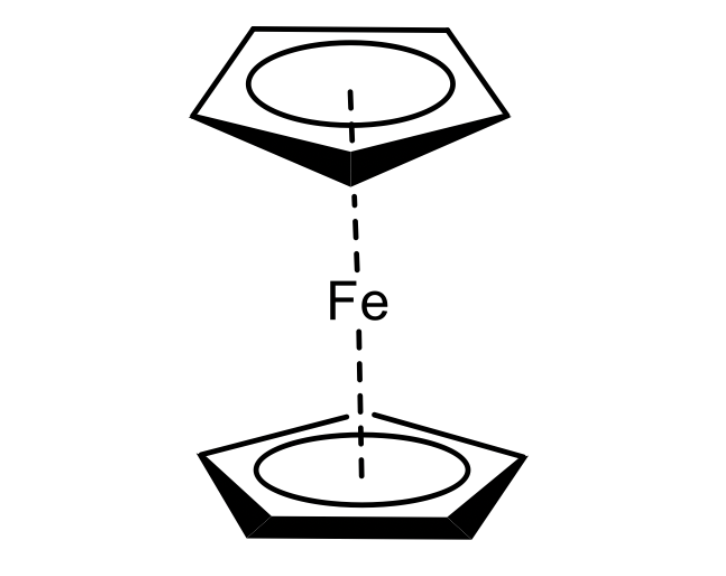
\includegraphics[width=.7\linewidth]{imagenes/estado_arte/teoria/ferroceno.png}
  \caption{}
\end{subfigure}%
\begin{subfigure}{.5\textwidth}
  \centering
  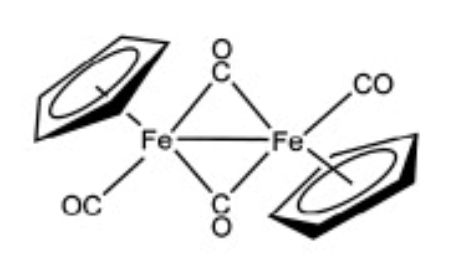
\includegraphics[width=.9\linewidth]{imagenes/estado_arte/teoria/derivativo_ferreoceno.png}
  \caption{}
\end{subfigure}
\caption{Representaciones 2D. \textbf{(a)} compuesto de ferroceno, que consta de un átomo de hierro central enlazado con 2 Cp; \textbf{(b)} derivativo del Dicarbonylcyclopentadienyliron. Imágenes extraídas de \cite{libreTextMetalocenos, artero_hydrogen_2008} respectivamente.}
\label{fig:metalocenos_ejemplos}
\end{figure}

\section{Herramientas o toolkits} \label{toolkits}

Existe una gran variedad de herramientas a la hora de trabajar dentro de la química computacional, tanto open-source como aplicaciones propietarias para las que son necesarias pagar una licencia de uso. La química computacional según comenté en el Capítulo \ref{introduccion}, se aplica en muchos ámbitos de la ciencia. Como tal, hay herramientas con propósitos muy distintos \cite{toolkits_recap}: 
\begin{itemize}
    \item Extensiones de navegador que mejoran el acceso a la información de las bases de datos \cite{safari_extensions}.
    \item Cálculos de propiedades fisicoquímicas (casi cualquier herramienta lo permite).
    \item Cribado virtual de moléculas como \textit{ChemAxon}, \textit{MOE}, \textit{LigandScout} o \textit{Forge}.
    \item Modelado y bocetado de moléculas como \textit{Marvin}, \textit{ChemDraw} o \textit{ChemDoodle}.
    \item Hojas de cálculo con análisis de datos químicos como \textit{Vortex}.
    \item Toolkits de propósito general con diversas funcionalidades básicas como \textit{OpenBabel} o \textit{RDKit}.
\end{itemize}
Las herramientas más complejas o relacionadas de alguna manera con la medicina suelen ser de pago. Para los objetivos de este proyecto se han tenido en cuenta los toolkits de propósito general mencionados anteriormente que son capaces de trabajar con SMILES.

\subsection{OpenBabel y RDKit}

Openbabel y RDKit son bastante parecidos en cuanto a sus funcionalidades, ambos permiten la manipulación de estructuras químicas, cálculos de propiedades moleculares, análisis de similitudes entre moléculas, generación de representaciones 2D y conversión entre distintos tipos de ficheros. Para elegir entre una de estas 2 herramientas, se han hecho pruebas iniciales en un notebook de Google Colab \cite{google_colab} (disponible el en GitHub de este proyecto).


RDKit por su parte, consigue representaciones 2D parecidas o mejores que las de OpenBabel para moléculas pequeñas y cuenta con mayores opciones de personalización del dibujo resultado \cite{rdkit_cookbook} haciéndolo más visual. Además, es más preciso a la hora de representar la estereoquímica, algo en lo que OpenBabel es bastante pobre. Vemos en la Figura \ref{fig:ejemplo_rdkit_vs_babel} un ejemplo con ambos paquetes software. Sin embargo, si se le exige un poco más a RDKit pidiéndole moléculas complejas no funciona del todo bien. Concretamente, cuando introducimos moléculas de organometálica no las lee correctamente aun siendo químicamente válidas. RDKit lleva a cabo un proceso de 'saneamiento' (\textit{sanitization}) \cite{rdkit_docbook} por el que, además de calcular algunas propiedades útiles (pertenencia de los átomos a anillos o hibridaciones), comprueba que la molécula de entrada es 'razonable'. Para RDKit, serán razonables las moléculas que cumplan la regla del octeto \cite{lewis2} y puedan representarse mediante las estructuras de Lewis de manera completa \cite{lewis_2013, lewis2}. Como hemos visto anteriormente, los compuestos de coordinación se rigen por otro tipo de sistema de valencia, y RDKit no es capaz de trabajar con esta clase de moléculas. De hecho, del set de moléculas del que dispongo para el proyecto, no es capaz de leer ningún código SMILES de los que fueron extraídos de SciFinder. Los SMILES de SigmaAldrich si los puede usar, pero más adelante en esta misma sección se explicará porqué estos no nos sirven.

\begin{figure}[h!]
\centering
\begin{subfigure}{.5\textwidth}
  \centering
  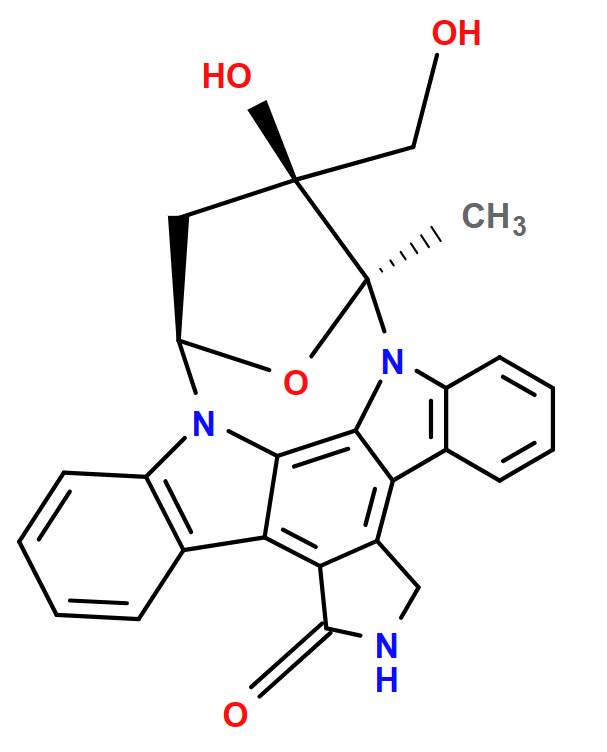
\includegraphics[width=.7\linewidth]{imagenes/estado_arte/Lestaurtinib_openbabel.png}
  \caption{OpenBabel}
\end{subfigure}%
\begin{subfigure}{.5\textwidth}
  \centering
  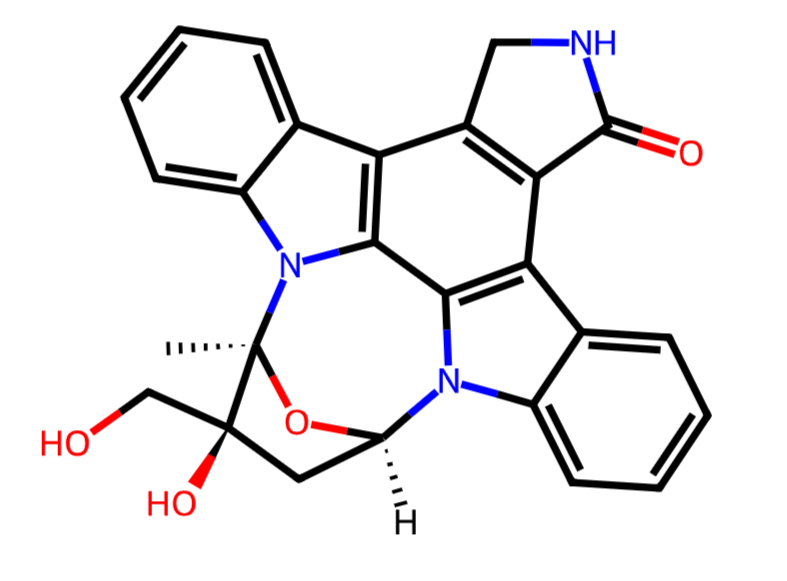
\includegraphics[width=.9\linewidth]{imagenes/estado_arte/Lestaurtinib_rdkit.png}
  \caption{RDKit}
\end{subfigure}
\caption{Representaciones 2D para el \emph{Lestaurtinib}, medicamento en estudio para el tratamiento de las leucemias agudas y algunos otros tipos de cáncer. \textbf{(a)} ha sido generado con OpenBabel; y \textbf{(b)} ha sido generado con RDKit.}
\label{fig:ejemplo_rdkit_vs_babel}
\end{figure}



OpenBabel por otro lado, ofrece más libertad en este sentido siendo capaz de leer todos los SMILES del set del que partimos. Pero en general, algo que hacen mal ambos paquetes es representar moléculas en 2D. Para moléculas convencionales, moléculas orgánicas o inorgánicas sencillas funciona bien, pero las organometálicas les supone un reto, y dada la escasa literatura en el tema (ver Sección \ref{revision_bib}), no dispongo de muchas referencias de las que partir.


En cuanto a los datos de partida contamos con 2 versiones de SMILES, los provenientes de SigmaAldrich y los de SciFinder. Siguiendo la comparación de la Sección \ref{motivacion} ambos SMILES son notablemente distintos, de hecho no se podrían considerar ni siquiera sinónimos ya que al de SigmaAldrich le faltan enlaces, y no llegan a codificar la misma molécula. Tanto es así que las cadenas SMILES que contienen desconexiones (representadas por el punto '.') no nos son para nada útiles. Al fragmentar la molécula estamos perdiendo los enlaces entre los átomos, una información muy valiosa para la mayoría de operaciones. Como se dijo antes, una molécula se suele almacenar principalmente identificando sus átomos y los enlaces entre sus átomos. Podríamos decir que se está perdiendo casi la mitad de la información acerca de la molécula, y dado que uno mismo no puede inventarse los enlaces, no es un buen SMILES para nuestros objetivos, ni para la canonización ni para el dibujado. En la Figura \ref{fig:dotted_smiles_vs_complete} vemos la diferencia entre la representación de un SMILES inconexo frente a uno con buena conectividad.


\begin{figure}[h!]
\centering
\begin{subfigure}{.5\textwidth}
  \centering
  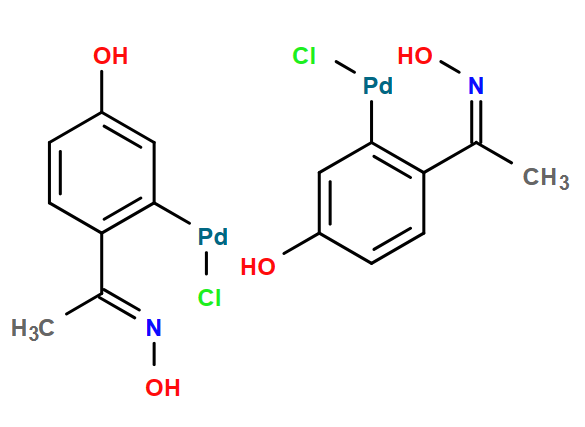
\includegraphics[width=.9\linewidth, frame]{imagenes/estado_arte/dotted_SA.png}
  \caption{}
\end{subfigure}%
\begin{subfigure}{.5\textwidth}
  \centering
  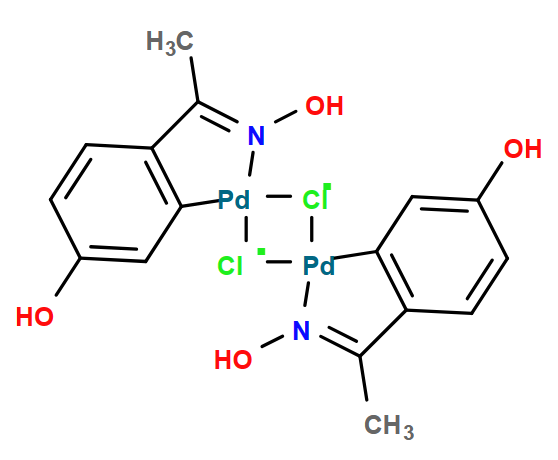
\includegraphics[width=.8\linewidth, frame]{imagenes/estado_arte/not_dotted_SF.png}
  \caption{}
\end{subfigure}
\caption{Representaciones 2D generadas con OpenBabel para el \emph{'Nájera Catalyst II'}. \textbf{(a)} SMILES con desconexiones extraído de SigmaAldrich; y \textbf{(b)} SMILES conectado extraído de SciFinder.}
\label{fig:dotted_smiles_vs_complete}
\end{figure}


\subsection{Herramientas de bocetado}
Existen herramientas tipo ChemDraw \cite{chemdraw_page}, que son las que los químicos e investigadores utilizan para dibujar manualmente las moléculas que luego añaden a sus publicaciones. Son este tipo de dibujos también los que probablemente podemos ver en algunas bases de datos como SigmaAldrich. En la Figura \ref{fig:chemdraw} se muestra su interfaz y algunas moléculas bocetadas.

\begin{figure}[h!]
    \centering
    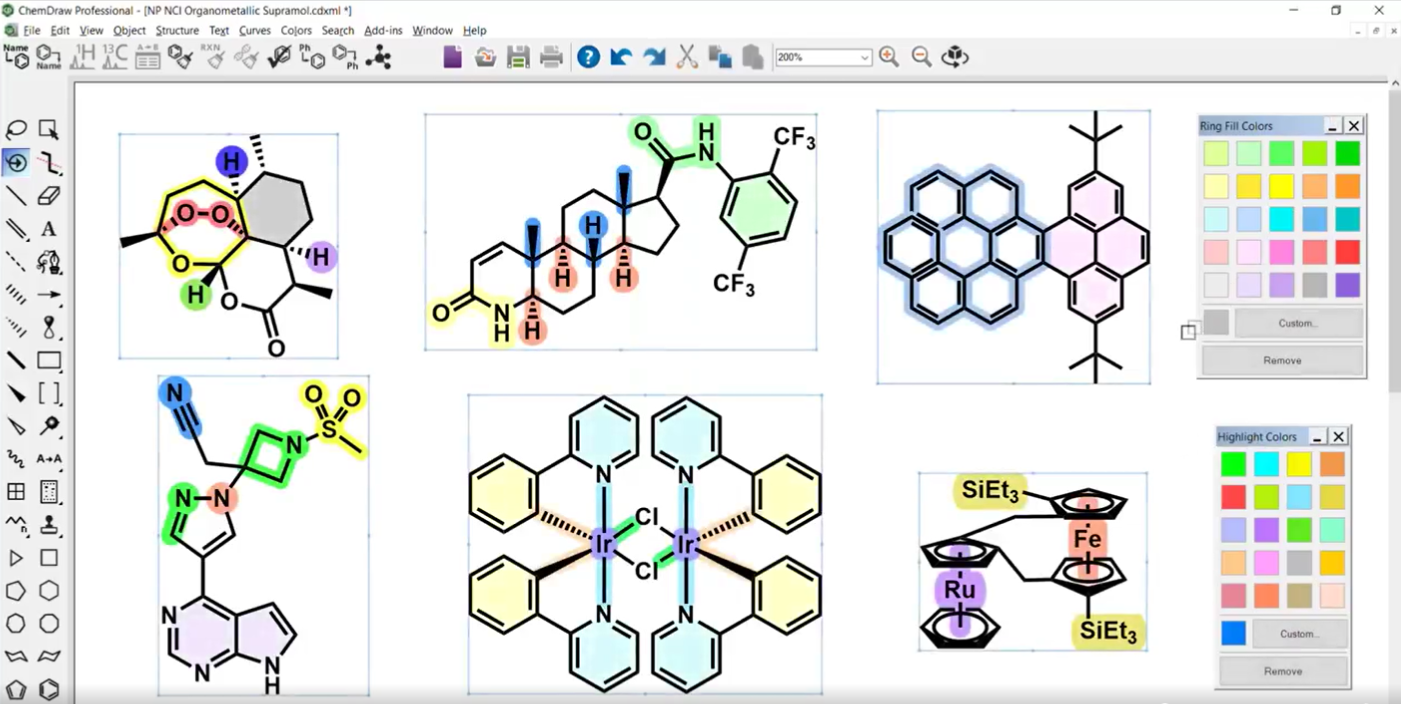
\includegraphics[scale=0.34]{imagenes/estado_arte/chemdraw.png}
    \caption{Interfaz de ChemDraw con algunas moléculas de prueba bocetadas. Imagen extraída de su página oficial \cite{chemdraw_page}}
    \label{fig:chemdraw}
\end{figure}

\subsection{Nomenclatura canónica} \label{estado:canon}
Como ya se ha visto, InChI proporciona una representación canónica para las moléculas, lo que permite una vinculación directa y unívoca entre las bases de datos. SMILES por otro lado complica este proceso. SMILES fue desarrollado en su momento como un software propietario por Daylight Chemical Information Systems (Daylight) \cite{daylight}, y desde su introducción a finales de los 80 se ha extendido como una norma de facto para representar estructuras moleculares. En base a esto y con el tiempo, se han escrito en varios lenguajes de programación muchos paquetes de software independientes que trabajan con SMILES\cite{opensmiles}.

Bien es cierto que hay cada vez más propuestas de cómo alcanzar una nomenclatura única \cite{weininger_smiles_1989, inchi1, nextmove_software_facto_nodate, baoilleach_we_nodate, universal_smiles} y ya existen algunas reglas definidas para la química orgánica a la hora de establecer prioridades entre los átomos y ordenar la molécula. Véase por ejemplo las \emph{'Reglas de Cahn-Ingold-Prelog'} aplicadas a enantiómeros \cite{cahn_specification_1966, prelog_basic_1982, NOMENCLATURA_R_S} para definir órdenes levógiros o dextrógiros (no abordaremos esto, excede el alcance del proyecto). Pero trasladar estas reglas a compuestos organometálicos es complicado, además de haber multitud de excepciones, en la mayoría de casos un mismo fragmento está enlazado por varios sitios al metal y hay que definir el átomo inicial por el que empezar a recorrer la molécula. Al final, cada paquete software implementa esta decisión de una manera diferente usando un algoritmo propio, obteniendo así lo que cada uno de ellos nombra como 'canonical SMILES', pero siguen siendo distintos entre ellos, por lo que no es canónico.

\subsection{Conclusiones}
Dicho todo lo anterior, durante las pruebas realizadas se ha podido comprobar y extraer las siguientes conclusiones:

\begin{itemize}
    \item Al representar la misma molécula con herramientas distintas, lo normal es que generen dibujos diferentes, en donde uno será mejor o más correcto que el otro.
    \item Para una misma molécula es probable que cada base de datos muestre una cadena SMILES diferente y una representación 2D distinta. De hecho, la imagen puede ni siquiera concordar con el SMILES que ofrecen, apareciendo en multitud de casos por ejemplo, un SMILES desconectado y una imagen con la molécula al completo (lo más seguro es que estén hechos a mano)
    \item Vistos los resultados de los SMILES de SigmaAldrich, para el resto del proyecto se asumirá que se trabaja con los SMILES de SciFinder, ya que dotan de mejor conectividad. 
    \item Debido a lo anterior, y como RDKit no soporta los datos de entrada, se utilizará la librería de OpenBabel para el proyecto.
    \item Hay diversos tipos de compuestos que no se describen bien mediante la representación de su grafo molecular, como los compuestos de coordinación. Su sistema de enlaces no se ajusta a la teoría de los enlaces de valencia, por lo que es complejo describir sus enlaces mediante relaciones 1 a 1 entre los átomos \cite{david_molecular_2020}.
    \item Moléculas complejas con multitud de ciclos o muchos enlaces al mismo átomo (generalmente un metal), OpenBabel genera unas representaciones 2D muy agrupadas, con los enlaces superpuestos y partes del dibujo unas encima de las otras, dificultando su entendimiento.
    \item Hasta el momento, no hay ningún sistema de canonizado que trabaje de manera eficiente con moléculas organometálicas.
    
\end{itemize}


Teniendo esto en cuenta y lo mencionado en la Sección \ref{motivacion}, en las siguientes secciones se dará pie a la implementación de una propuesta de nomenclatura canónica para moléculas organometálicas y la mejora del dibujado de las mismas con OpenBabel.





